
\section{PiP Tasks}

This section will describe how PiP tasks are created in a simple way
and how PiP tasks works in the different way from the process (using
\term{MPI}) and thread (using \term{OpenMP}) creations.

\subsection{\PIPKW{pipcc} and \PIPKW{pip-exec} Commands}
\label{sec:pipcc-exec}

The first example is  the well-known C program ``hello world'' listed
below; 

\lstinputlisting[style=program, caption={Hello World},label=prg:hello]
                {tasks/examples/hello.c}

As you can see, this program is exactly the same with the normal C
program. If this program is compiled with the \pipcmd{pipcc} command,
then this program can run as a normal C program or as a PiP task by
using the \pipcmd{pip-exec} command.

\lstinputlisting[style=example, 
  caption={Hello World - Compile and Execute}, label=out:hello]
                {tasks/examples/hello.out}

The \pipcmd{pipcc} command is written as a shell script to call a real
C compiler with appropriate options, such as {\tt -I}, {\tt -L} and so
on. If the {\tt --silent} option is omitted, then you will see the
options how \pipcmd{pipcc} script calls the backend C/C++ compiler.

The \pipcmd{pip-exec} command in this example is to execute an
executable file as PiP tasks, not as a normal Linux process.

This example does not show how the hello program behaves differently
between the process and PiP task. The next section wil discuss on this
point.

\subsection{Comparing MPI, OpenMP and PiP}

To explain the difference between process and PiP task, we slightly
modify the ``hello world'' program as below;

\lstinputlisting[style=program,
  caption={Hello World having a static variable},
  label=prg:hello-var] {tasks/examples/hello-var.c}

Now the ``Hello World'' program has a static variable
{\tt x} and its address is printed out with the ``Hello World''
message. The \pipcmd{pip-exec} command may take an option to specify
the number of PiP tasks to be created and executed in parallel. In the
following execution example, the number of three (3) is
specified. Additionally, the output of the same {\tt a.out} execution
using \term{MPI}. It should be noted that the ``Hello World'' program runs in
parallel with \pipcmd{pip-exec} and \mpi{mpiexec}. 

\lstinputlisting[style=example, 
  caption={Hello World with a static variable - Compile and Execute},
  label=out:hello-var] {tasks/examples/hello-var.out}

The first execution of {\tt a.out} shows that the variable {\tt x} is
located at the address of {\tt 0x555555601030}\footnote{For
simplicity, we disabled ASLR (Address Space Layout Randomization) in
this example.}. This situation is the 
same with the \term{MPI} execution\footnote{MPICH implementation where each
MPI rank has its own address space.}. However, the locations of the
variable {\tt x} executed as PiP tasks are all different.
This is because PiP tasks share the same address space but \term{MPI} does
not. Readers may notice that threads also share the same address
space and wonder the difference between PiP and \term{OpenMP}. The example
below is the \term{OpenMP} version of the ``Hello World'' with a static
variable. 

\lstinputlisting[style=program,
  caption={Hello World in OpenMP},
  label=prg:hello-var-omp] {tasks/examples/hello-var-omp.c}

The execution output of program~\ref{prg:hello-var-omp} is shown
below. Here, the addresses of variable {\tt x} are the same in \term{OpenMP}
and \term{MPI} executions. However, the addresses of the variable with PiP
execution are different pairs. 

\lstinputlisting[style=example, 
  caption={Hello World in OpenMP, PiP and MPI - Compile and Execute},
  label=out:hello-var-omp] {tasks/examples/hello-var-omp.out}

Figure~\ref{fig:tasks:hello-var-omp} explains these differences. In
\term{OpenMP}, the \term{OpenMP thread}s share the same address space
and variable {\tt x} is shared among threads. In \term{MPI}, each
\term{MPI process} has its own address space and two (2) threads run
in each address space and share the variable in the same \term{MPI
  process}. In PiP, all PiP tasks share the same address space,
however, each PiP task has its own variables and thread 0 and 1 share
the variable in the same PiP task, but not sharing the variables in
the different PiP task (Figure~\ref{fig:tasks:hello-var-omp}).

\begin{figure}[ht]
\centering
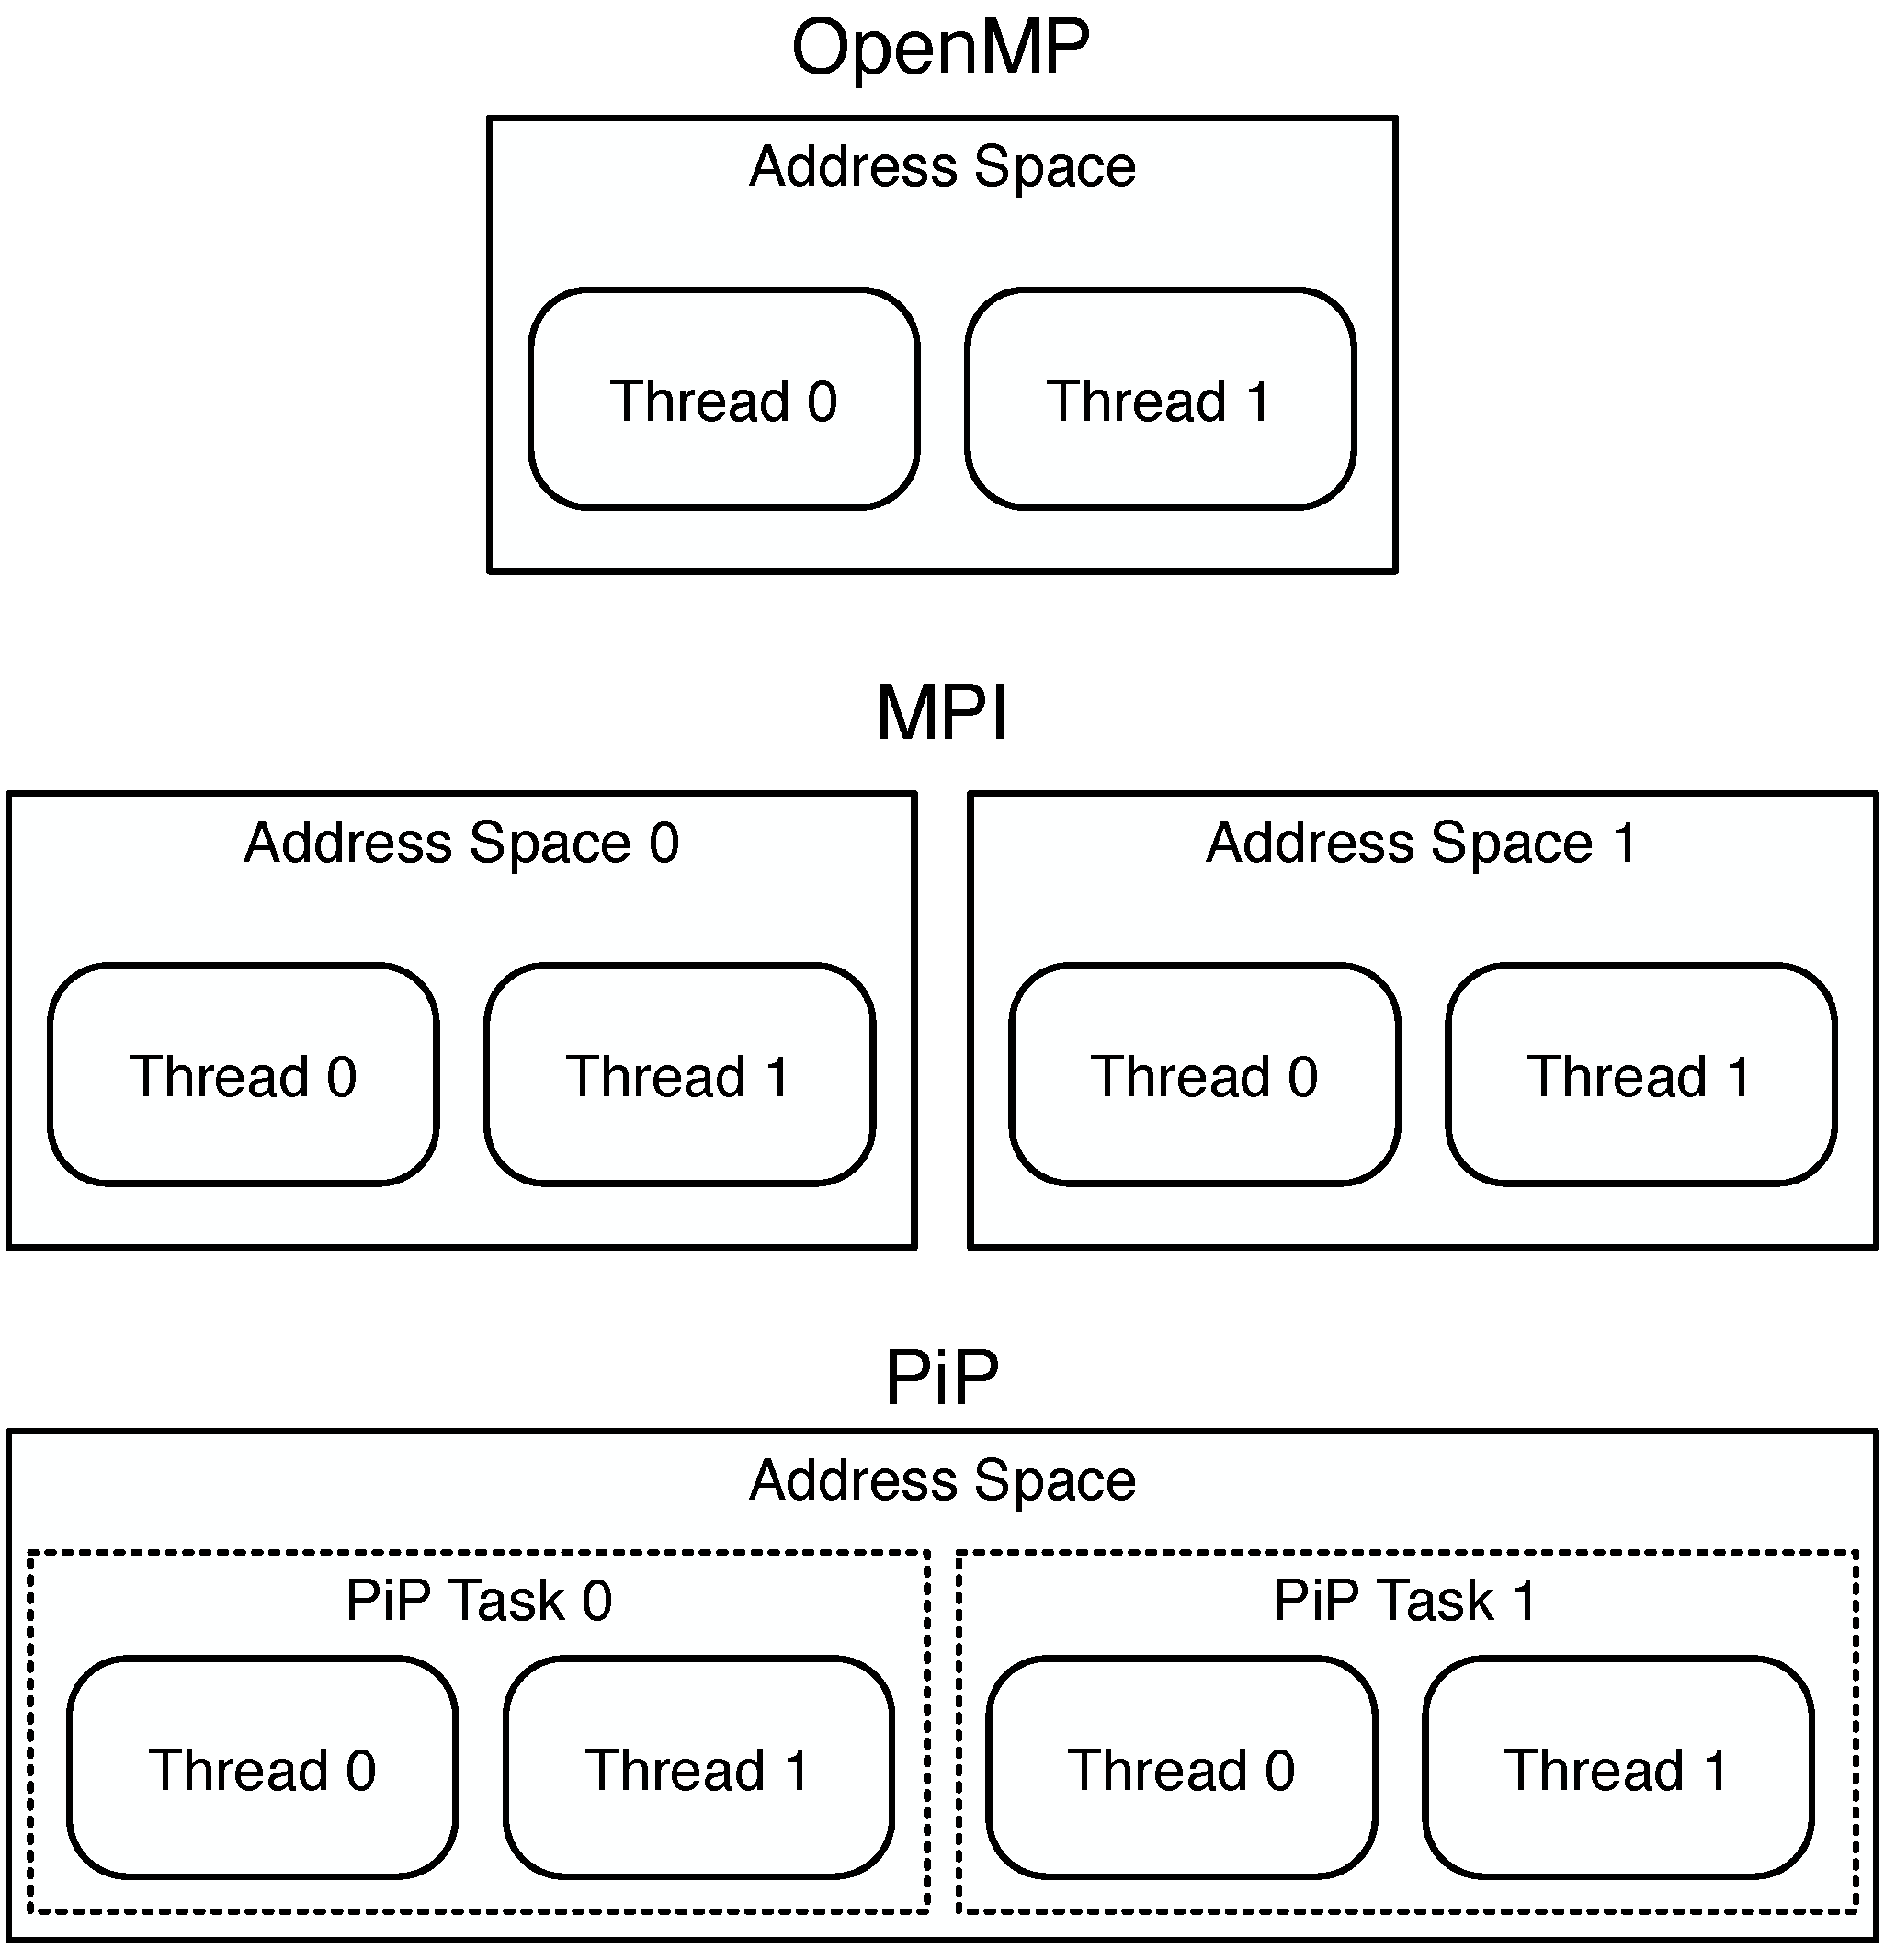
\includegraphics[width=0.7\columnwidth]{tasks/Figs/AddressSpace-OpenMP-MPI-PiP.pdf}
\caption{Differences of OpenMP, MPI and PiP}
\label{fig:tasks:hello-var-omp}
\end{figure}

In the conventional process model and thread model, static variables
are associated with an address space. Thus, each process has its own
static variables and threads running on the same address space share
the same static variables. In the PiP execution model, each PiP task
is guaranteed to have its own static variable set, decoupling from the
address space while maintaining the address space sharing. This is
called {\bf \term{variable privatization}}. 

This nature of PiP, privatized variables and sharing an address space,
makes it easy to exchange information among PiP tasks while
maintaining the independence of each PiP task execution. 
So far, it is shown that the ``Hello World'' program can run as PiP
tasks in parallel, but this program is so simple and no information
exchange among PiP tasks. In the next section, we will show how
information can be exchanged among PiP tasks.

\subsection{Export and Import}

Sharing an address space means that data owned by a PiP task
can be accessed if the address of the information to be exchanged is
known. A PiP task can publish the address of the data to be shared
and the other PiP task(s) can get the published address. 

Firstly, each PiP task has {\PIPID} to distinguish from the
others. A PiP task can export an address so that the other PiP tasks
sharing the same address space can import the address by
specifying the {\PIPID} who exported. 

\lstinputlisting[style=program,
  caption={Export and Import ({\tt export-import})},
  label=prg:export-import] {tasks/examples/export-import.c}

In this program, a PiP task having {\PIPID} of zero (0) export
the address of the variable {\tt x} by calling
\pipfunc{pip_named_export()} after setting the value of {\tt
  argv[1]}. The 
other PiP tasks import the exported address by the PiP task 0 by
calling \pipfunc{pip_named_import()} function. Below is an execution
result of this program. As shown, the exported value by PiP task 0 can
be seen by the other PiP tasks. 

\lstinputlisting[style=example, 
  caption={Execution of Export and Import},
  label=out:export-import] {tasks/examples/export-import.out}

The \pipfunc{pip_named_export()} function publishes an address with
the given name. The \pipfunc{pip_named_import()} function
blocking-waits until the named address on the specified PiP task by
{\PIPID}. It is not allowed to export an address having the same
name twice or more to update the address, because this leads to a race
condition. 

Almost all functions provided by the PiP library return an integer
value as an error code. The return code of zero (0) means success. This
error code is the same with the ones defined by Linux. In
the examples so far and hereinafter, the returned code is not checked
because of simplicity and readability. 

In \term{MPI}, it is not allowed to access the data owned by the other
processes in the same node. Communication is the only way allowed in
\term{MPI}\footnote{Strictly speaking, some \term{MPI} implementations based on the
thread model may allow this. Major \term{MPI} implementation, such MPICH,
Open MPI, and many other \term{MPI} implementations provided by vendors are
based on the process model and there is no way to access data owned by
the other \term{MPI process}.}. Basically, communication involves some form
of data copying (done by software or hardware). Data copying consumes
time, power and memory. 

